\documentclass[12pt,preprint]{aastex}
\usepackage{listings}

\begin{document}

\title{SUGGESTIONS FOR LAB REPORTS---\today}

\tableofcontents

\section{A Typical Outline for a Scientific Paper}

A typical scientific paper is divided into sections, subsections, and
subsubsections. The global outline for a typical scientific paper looks
like the following. Note, however, that there are wide variations from
this, which depend on content, subject matter, and individual
style. 

In the typical organization shown below, the most important sections are
numbers 4, 5, and 6 below. This course emphasizes datataking, data
analysis, and data intepretation. 


\begin{enumerate}

\item Title. Should encapsulate the contents and meaning.

\item Abstract. A short summary of the paper including the most important
  results.  Purpose is to tell a prospective reader whether it is worth
  spending time and effort on the article.
  
\item Introduction. Sets the context: summary of the current state of
  knowledge, how that state can be improved, what this work does to
  advance the field. What did you hope to accomplish? Briefly, what did you
  accomplish? 

\item Observations or Experiments. What you observed, who did it, when you
  did it, what equipment you used, how you recorded data, any particulars
  or peculiarities.

\item Data Analysis. The theory according to which you analyze the data,
  how you actually did the analysis, the results of your analysis. Provide
  the essential numbers---the distillation of your original data (often
  millions of numbers) into a set of essential numbers or results. This is
  what we mean by ``data reduction''!

\item Interpretation. What the results mean in terms of astrophysics or
  your previous state of knowledge. How your results relate to specific
  issues that were mentioned in the introduction.

\item Because this is a class, and because you are working in groups, we
  need a section that summarizes who did what. The idea is that each
  individual will participate in enough data-gathering activities to
  learn and understand how and what's being measured, and make a useful
  contribution to the group's efforts. In addition, each individual
  should write appropriate portions of the reduction and display
  software. In order for me to understand your progress and
  contributions, you should have a section of your report {\bf (1)}
  describing your contributions; {\bf (2)} listing what software you
  wrote and which plots you yourself made; {\bf (3)} stating who wrote
  other software and other plots that you used; {\bf (4)} listing your
  contributions to other software written by the group; {\bf (5)}
  providing me with the subdirectories where the various pieces of
  software reside so I can take a look at it if necessary. The
  permissions on these files should allow me to read them.

I would also like you to describe problems or difficulties, and aspects
that remain confusing or unclear. Also, your descriptions about who did
what should be accurate and not exaggerated. Making these explicit can
help us address the issues so that we achieve the overall course goals
of making you very well-versed in experimental and laboratory work.
 
\item Conclusion. A summary of important results and points made in the
  paper, including pointing to the particular sections so that the reader
  can easily learn more detail. What aspects are lacking? How would
  you have done things better? Prospects for future work.
  

\end{enumerate}

\section{Scientific and Interpretive Issues}

	These are {\it most important} because they related directly to
your scientific and experimental work and interpretation. 
\begin{itemize}

\item When you derive a result or calculate something it's important to
be {\it self-critical}. This is known as a {\it reality check}. Various forms
of reality check include the following (a limited list):
\begin{enumerate}

	\item Generate fake data. Run your software on them ({\it note
the plural use of ``data''!}) and check for consistency. 

	\item When doing a least-squares fit, plot the {\it data},
overplot the {\it fitted curve}, and plot the {\it residuals}. The data
and fitted curve should look similar. The residuals should exhibit no
systematic trends and should look like noise clustered around zero. If
not, why not?

	\item Before deriving a result with fancy numerical techniques
you should first make a guess, using your physical intuition, about what the
answer is. If your fancy numerical technique gives something wildly
different, then  \begin{enumerate}

	\item Your physical intuition is no good, which means you don't
understand the basic fundamentals. 

	\item Your numerical technique or software is no good.
\end{enumerate}

\noindent Which is it? (Or is it both????) Talk to people, ask
questions, or whatever, but {\it resolve these discrepancies!}

\end{enumerate}

	\item When you plot some data, {\it look at the plot and think
          about what you see}.  For example, when observing the Sun with
          the interferometer on Campbell Hall's roof, the Campanile
          shadowed the dishes and the signal went away for some time.
          Ask yourself: what happened to the data during that time? In
          your lab report, such things are worth comments!

\item Abstracts should contain essential information---{\it including the
important numbers that you derive}. 

\end{itemize}

\section{ Grammar, etc.}

	Some grammatical-type issues: \begin{itemize}

	\item The word `data' is {\it plural}. Use it as you would use
the word `datapoints'. The singular of data is {\it datum}. Use it as
you would use the word `datapoint'. For example: \begin{enumerate}

	\item The data {\it indicate} (not {\it indicates!}) that the
system doesn't work\dots Similar to saying ``The datapoints
indicate\dots''

	\item This datum {\it is} a bad measurement and we will discard
it.  
\end{enumerate}

	\item Capitalize proper names. This includes `Fourier', `Gauss'
or `Gaussian', `Sun', `Moon', `Orion', etc.

	\item Check spelling! From the UNIX prompt, type

\begin{verbatim}
ispell -t mylab.tex
\end{verbatim}

\noindent which runs an interactive spell checker. The \verb$-t$ means
``ignore TEX-related commands''. Spell checking isn't a panacea because a
typo can produce a properly spelled word that isn't appropriate.
Example: ``These data are like ship.''

\end{itemize}

\section{ Plotting/Python Issues} \label{plotting}

	Some plotting- or Python-related issues: \begin{itemize}

	\item Axis labels and annotations on plots need to be large
enough to be legible.  Also, you really ought to use nice fonts: don't
underestimate the value of good looks! Figure \ref{simple} illustrates
the difference between the following two plotting routines.

\lstinputlisting[language=Python]{plot_simple.py}

\lstinputlisting[language=Python]{plot_nicer.py}

\begin{figure}[b!]
\begin{center} 
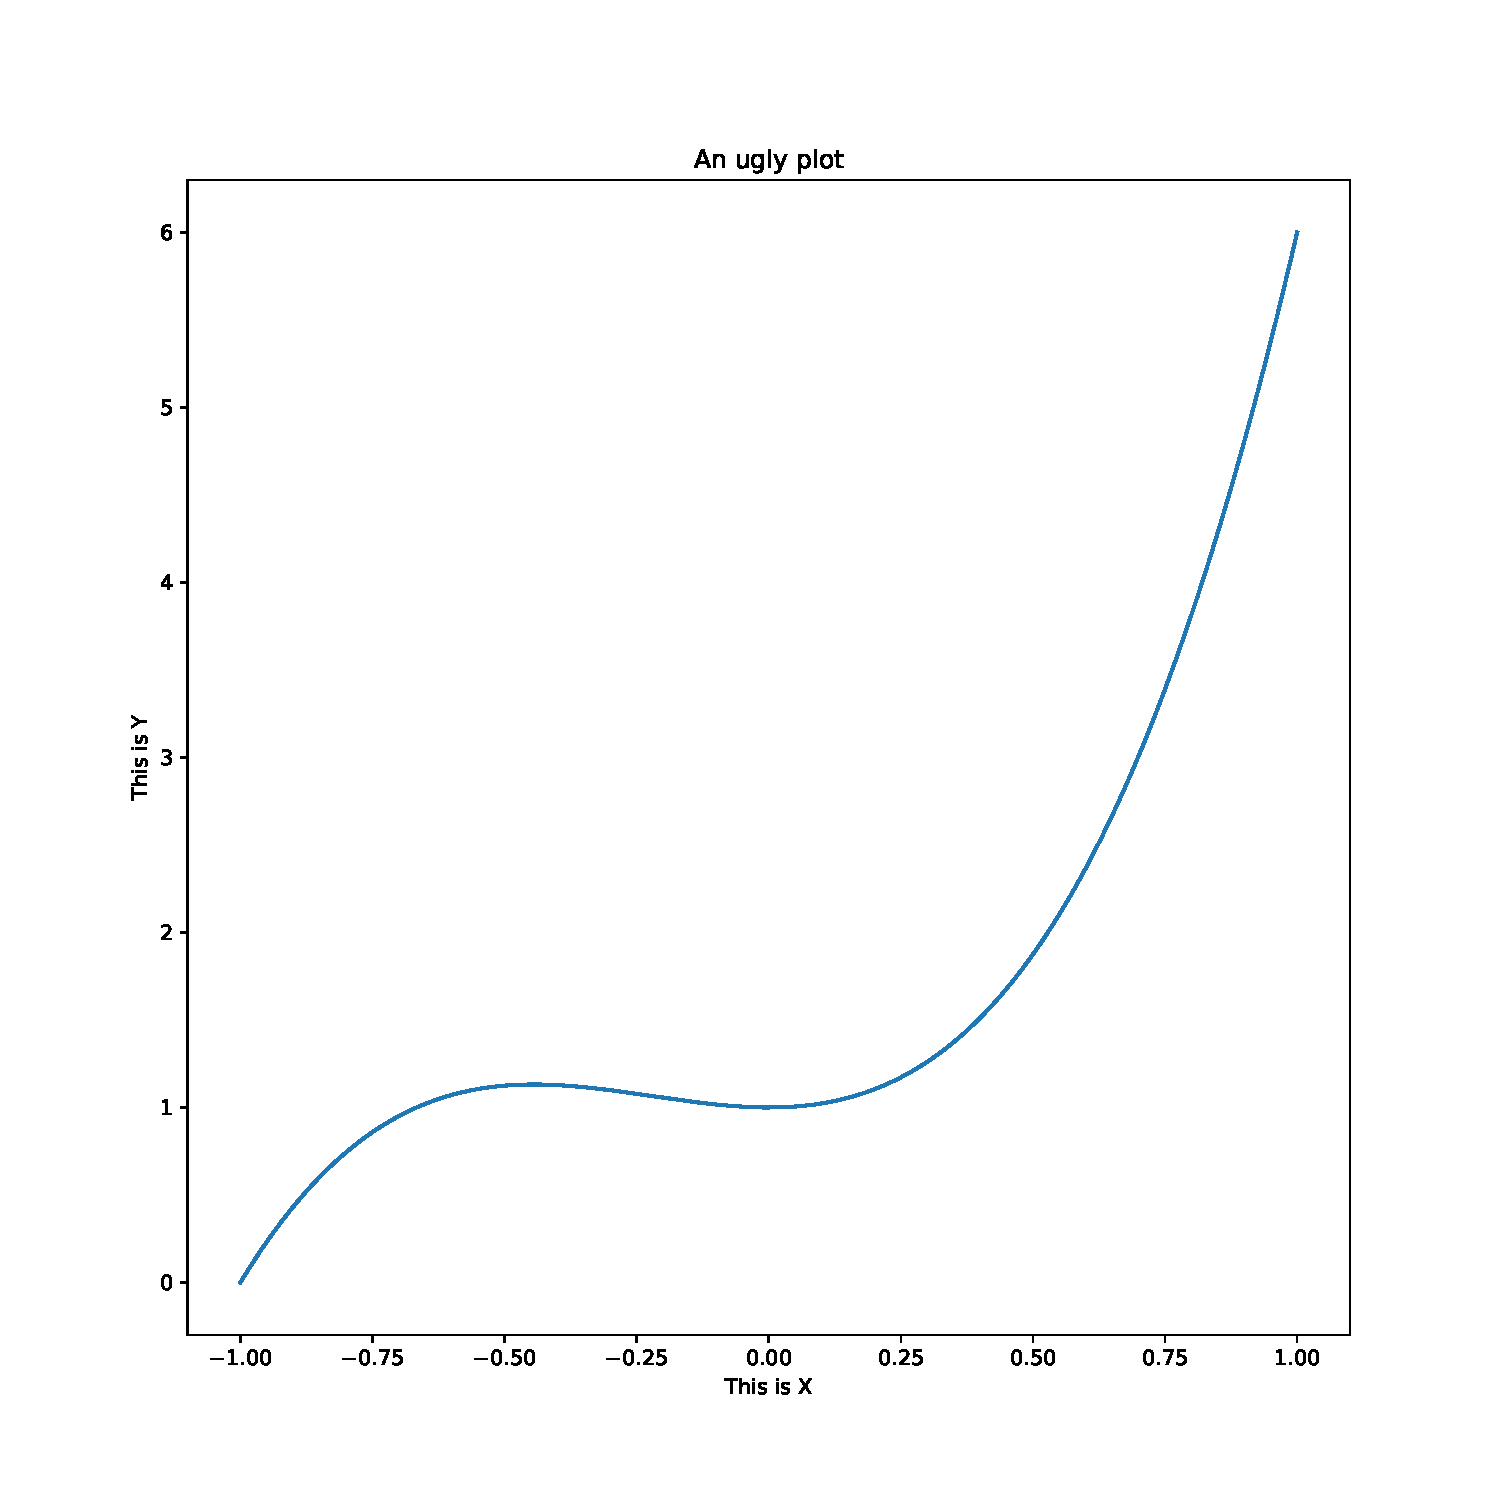
\includegraphics[width=3in]{simple.pdf}
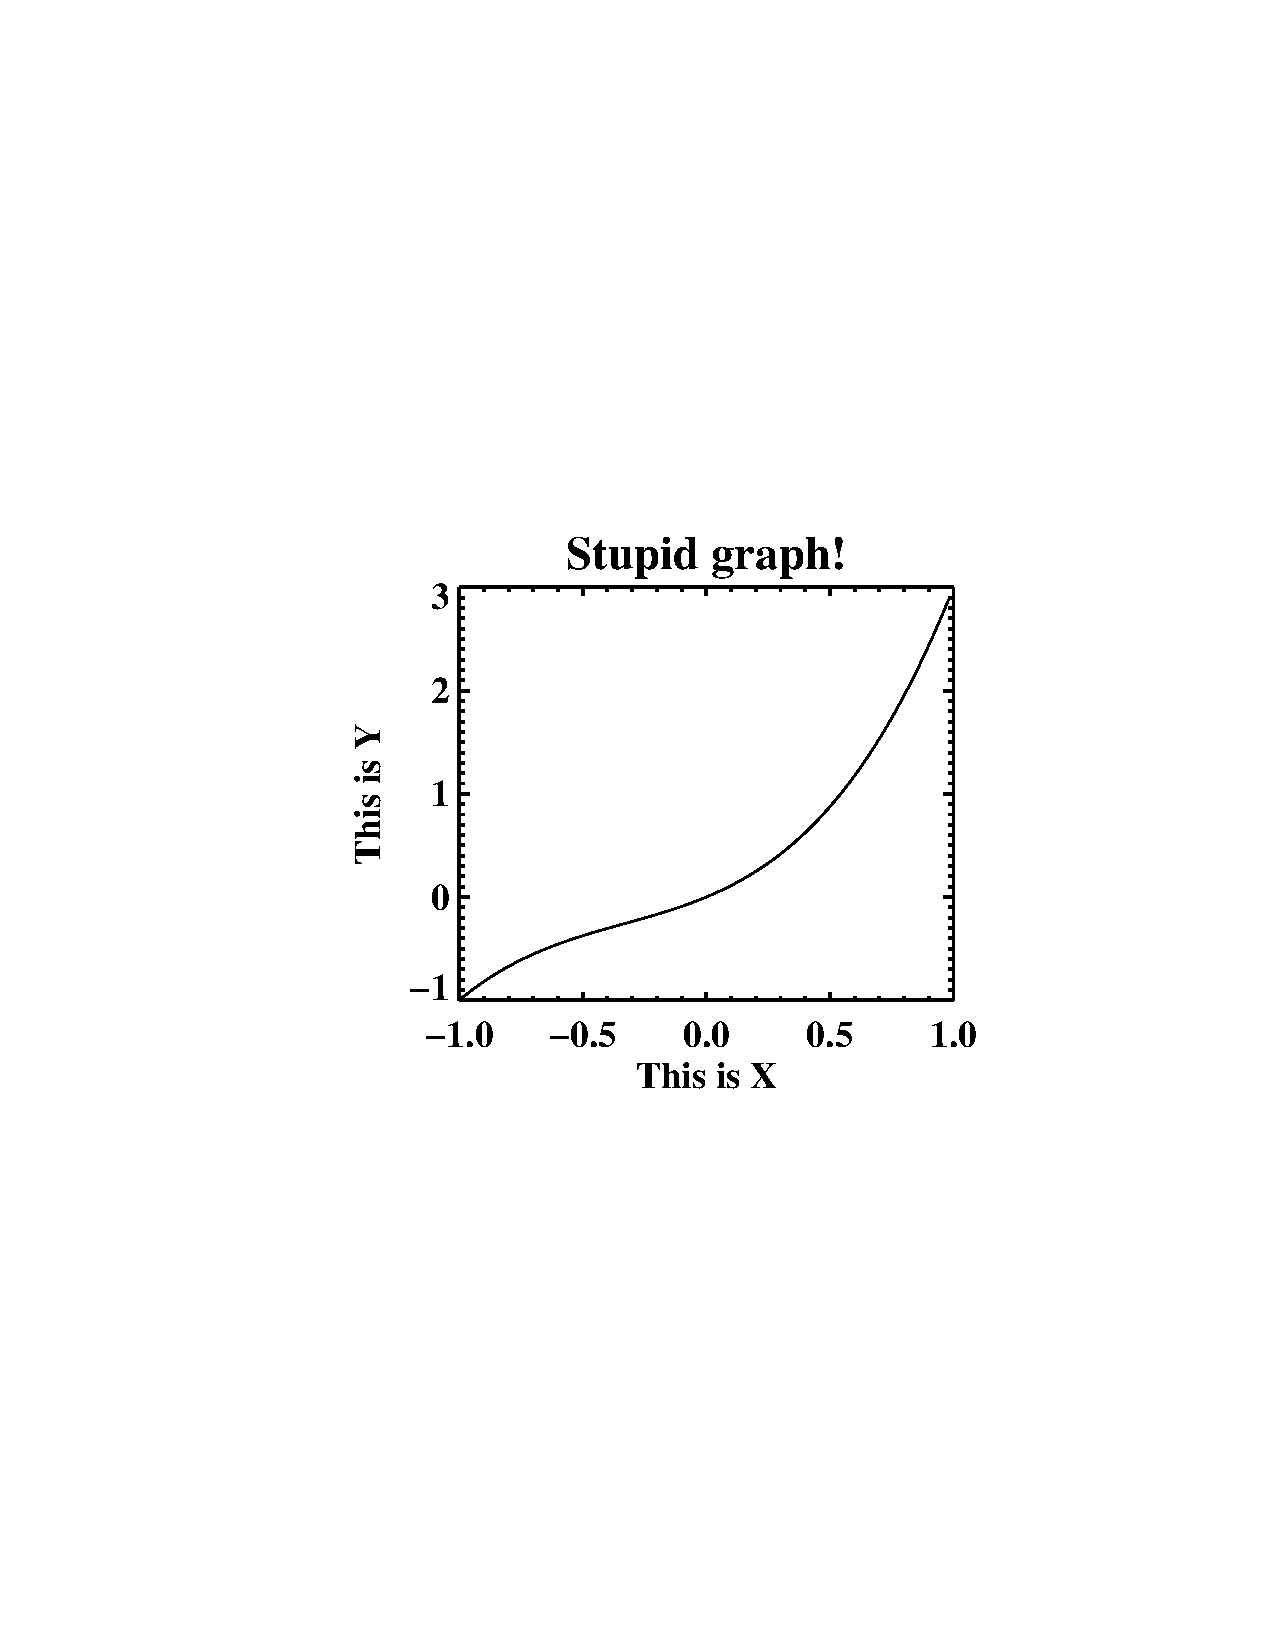
\includegraphics[width=3in]{nicer.pdf}
\end{center}
\caption{Left: Titles are too small, lines too thin, font doesn't look
good. Right: Nicer! (But it could be even nicer!!) See \S
\ref{plotting}.  \label{simple}}
\end{figure}
                                                                        

\item When plotting datapoints, it's usually a good idea to plot the
  points themselves, which you'd do with the keyword \verb$marker='o'$, for
  example \footnote{Or any other symbol matplotlib supports}
    Sometimes you also want to connect the datapoints
  with lines, which you do with \verb$linestyle='solid'$.

\item When you do a least squares fit, you want to overplot the
  datapoints with a fitted curve; to do this, plot the datapoints
  (e.g.\ {\tt plot(x, data, 'ko')}) and then plot the fit over it
  in color (e.g.\ {\tt plot(x, fit, 'r-')}), but almost 20\% of human males are red/green
  colorblind, so out of consideration you should overplot with a
  different line style (e.g.\ {\tt plot(x, fit, 'k--')}) or both
  ({\tt plot(x, fit, 'r--')}).

\item If you want to evaluate fancy mathematical functions you don't
need to use Mathematica.  Python (specifically, scipy) has all those functions too.  For example,
from the IPython prompt, type \verb$scipy.special.gamma?$ to get info on the Gamma
function.  A software language is just that---a {\it language}---and the
more proficiently you speak it, the better off you are.  

\item Python's matplotlib is able to use TeX markup.  This means you can put TeX into
titles and axis labels: (e.g. {\tt xlabel(r'\$\verb$\$nu\$ [MHz]')}).  Because '\verb$\$'
is an escape character in Python strings, you'll either need to use a double backslash (\verb$'\\nu'$)
or use raw strings (\verb$r'\nu'$).

\end{itemize}

\section{TEX hints}

	Some TEX hints: \begin{enumerate}

	\item Mathematical convention says: usually, write
$(R^2-x^2)^{1/2}$ instead of $\sqrt{R^2-x^2}$.  In TEX, the scripts are
\verb&$(R^2-x^2)^{1/2}$& and \verb&$\sqrt{R^2-x^2}$&. 

	\item When you're doing complicated parenthetical expressions,
it's nice to use embedded sizing. TEX does this automatically for you:
instead of the not-very-elegant

$$x=\cos[2\pi(\frac{B_y}{\lambda}\cos(\delta))\sin(h)]$$

\noindent you can write

$$x=\cos\left[2\pi\left(\frac{B_y}{\lambda}\cos(\delta)\right)\sin(h)\right]$$

\noindent The scripts for these are

\begin{verbatim} 
$$x=\cos[2\pi(\frac{B_y}{\lambda}\cos(\delta))\sin(h)]$$

and

$$x=\cos\left[2\pi\left(\frac{B_y}{\lambda}\cos(\delta)\right)\sin(h)\right]$$
\end{verbatim}

\noindent Note the (double) use of \verb$\left[$ and \verb$\right$] . 
Also, note the Roman letters for the trig function, i.e.\ convention
prefers $\cos(ha)$ instead of $cos(ha)$; we accomplish this in TEX by
writing \verb$\cos(ha)$ (note backwards slash in \verb$\cos$) instead of
\verb$cos(ha)$. 

\item You can print a Table of Contents by writing
\verb$\tableofcontents$ in your TEX document (usually at the beginning,
but you can do it anywhere). This is very helpful when
organizing your lab report into sections and subsections.

\item You can get the proper looking quotes, either `single' or
``double'', by writing \verb$`single'$ or \verb$``double''$ . 

\item You can get a proper ``times'' sign, as in $2 \times 3$, using
\verb=$2 \times 3$=. 

\item You can get equations numbered 1a, 2b, and 3c instead of 4, 5,
and 6 by using the \verb$mathletters$ environment like this:
\begin{mathletters}
\begin{equation}
x = \sin (y)
\end{equation}
\noindent and then you can insert as much text as you want and\dots
\begin{equation}
z = \tan (y)
\end{equation}
\begin{equation}
u =  y^{1/2}
\end{equation}
\end{mathletters}
by typing the following:
\begin{verbatim}
\begin{mathletters}
\begin{equation}
x = \sin (y)
\end{equation}

\noindent and then you can insert as much text as you want and\dots

\begin{equation}
z = \tan (y)
\end{equation}
\begin{equation}
u =  y^{1/2}
\end{equation}
\end{mathletters}
\end{verbatim}

\item And finally, you can insert things verbatim into TEX, without the
TEX translations, by using \verb=\verb$verbatim into TEX$= (all must be
on one line) or, for multiple lines, get into the \verb$verbatim$
environment by typing

\begin{verbatim}
\begin{verbatim}
Now we are in the verbatim environment
Here is a multiple line situation
\end{verbatim}
\verb$\end{verbatim}$
\end{enumerate}

\section{Grades \dots}

 Your primary job in the report is to convince me that you understand
 what you're doing and have incorporated the lab's goals into your
 psyche.  So look at the list of goals in the lab handout. The ideal
 report would address each goal. Then look at the above sections in this
 handout and incorporate them in your report.

When covering a given topic, include supporting data with figures,
 tables, and discussion to the extent that they are illustrative and
 educational for the reader. Don't include material simply because `it's
 there' or to make your report longer. What matters is clarity. And
 being concise is a virtue. For example, instead of including every
single plot you made, a well-considered and
 well-selected set of plots---annotated, labelled, presented neatly, and
discussed in the text---shows that you understand what's important.

Sometimes your lab activities are relevant to aspects in world outside
 the undergrad lab. For example, in discussing Fourier transforms, you
 might think about their usefulness in other science areas, for example
 seismology or the characterization of music. Or when we cover
 waveguides, does this resonate with other courses in Physics,
 e.g.\ Physics 110?

If your results seem discrepant with expectation, how do you resolve
this? You might think that  you have to `get the right answer'. But in
research, particularly experimental research, the `right answer' may
differ depending on the experimental conditions, such as signal levels
or interfering signals. Should you hide or minimize your puzzlements or
mistakes so that I'll think you're really smart? Or should you emphasize
your problems or difficulties  by showing them explicitly, sometimes
even to the extent of having a separate section that discusses them?
Which way will you learn more? Which way will I appreciate?

If you can make your report interesting to me as a reader, then that in
 itself is a marker of your good understanding. Moreover, I'm more
 likely to pay attention to what you're saying!

\end{document}

